\textbf{Abstract} Reproduction of {\em N. P. Rougier. “LOUPE.” In: Tremplin Micro 19 (Mar. 1988), pp. 60–61} for the \href{https://rescience.github.io/ten-years/}{Ten Years Reproducibility Challenge}.

\section*{Introduction}

I published my very first (non-scientific) article\supercite{rougier:1988} in a
French Magazine named ``Tremplin Micro'' in 1988, 32 years ago. It was a
program written
in \href{https://en.wikipedia.org/wiki/Applesoft_BASIC}{Applesoft Basic} that
zoomed out a 21$\times$21 pixels area of an image by a factor 4 (not very
impressive by 2020 standards). As written in the original ``cover'' letter I
sent, the zoom was also very slow. At that time, I was learning 6502 assembler
but I was not proficient enough to write the program using it. Thirty-two years
might appear a relatively small lapse of time compared to Human history, but
for digital computer history, this is actually huge, almost half of its
history. Imagine that the Apple~//e was using a 6502 microprocessor with a
8-bits data bus, had 64Ko of RAM and the speed was barely 1Mhz. The text modes
were 40 or 80 columns, and the video modes include a standard graphic mode
(140x96 pixels, 16 colors) or an impressive high-resolution mode (280x192
pixels, 6 colors). Despite these apparent limitations, the Apple~//e has been a
very popular machine complemented by an extended software library.
%%
\begin{figure}
{%% <-- begin a group to make \fboxsep=0pt local
\fboxsep=0pt
\fbox{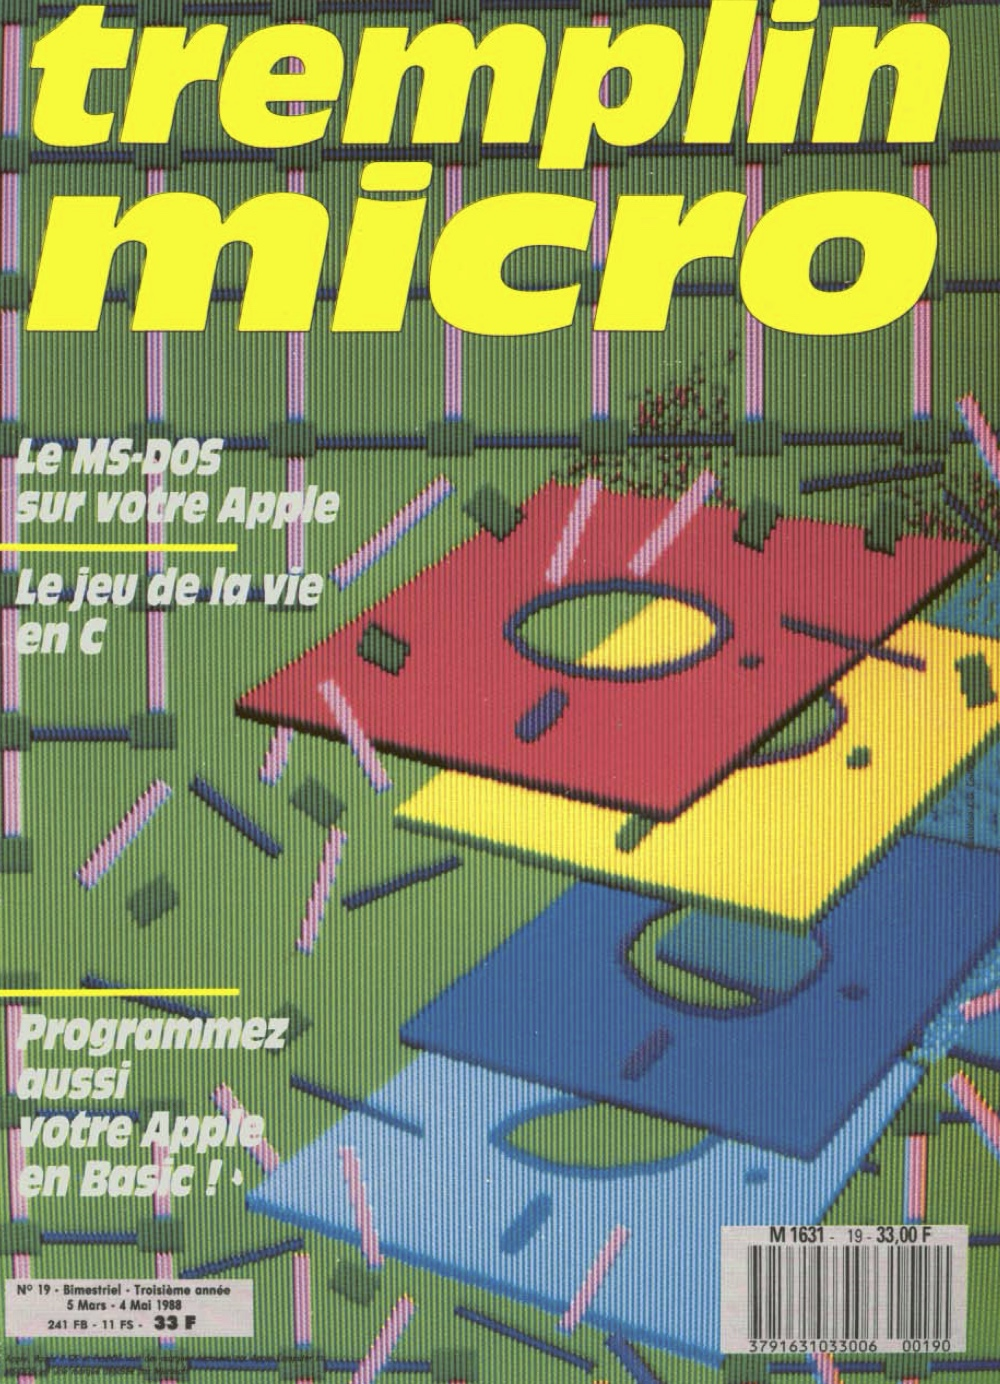
\includegraphics[width=.325\textwidth]{Tremplin-Micro-19-p1.jpg}}
\fbox{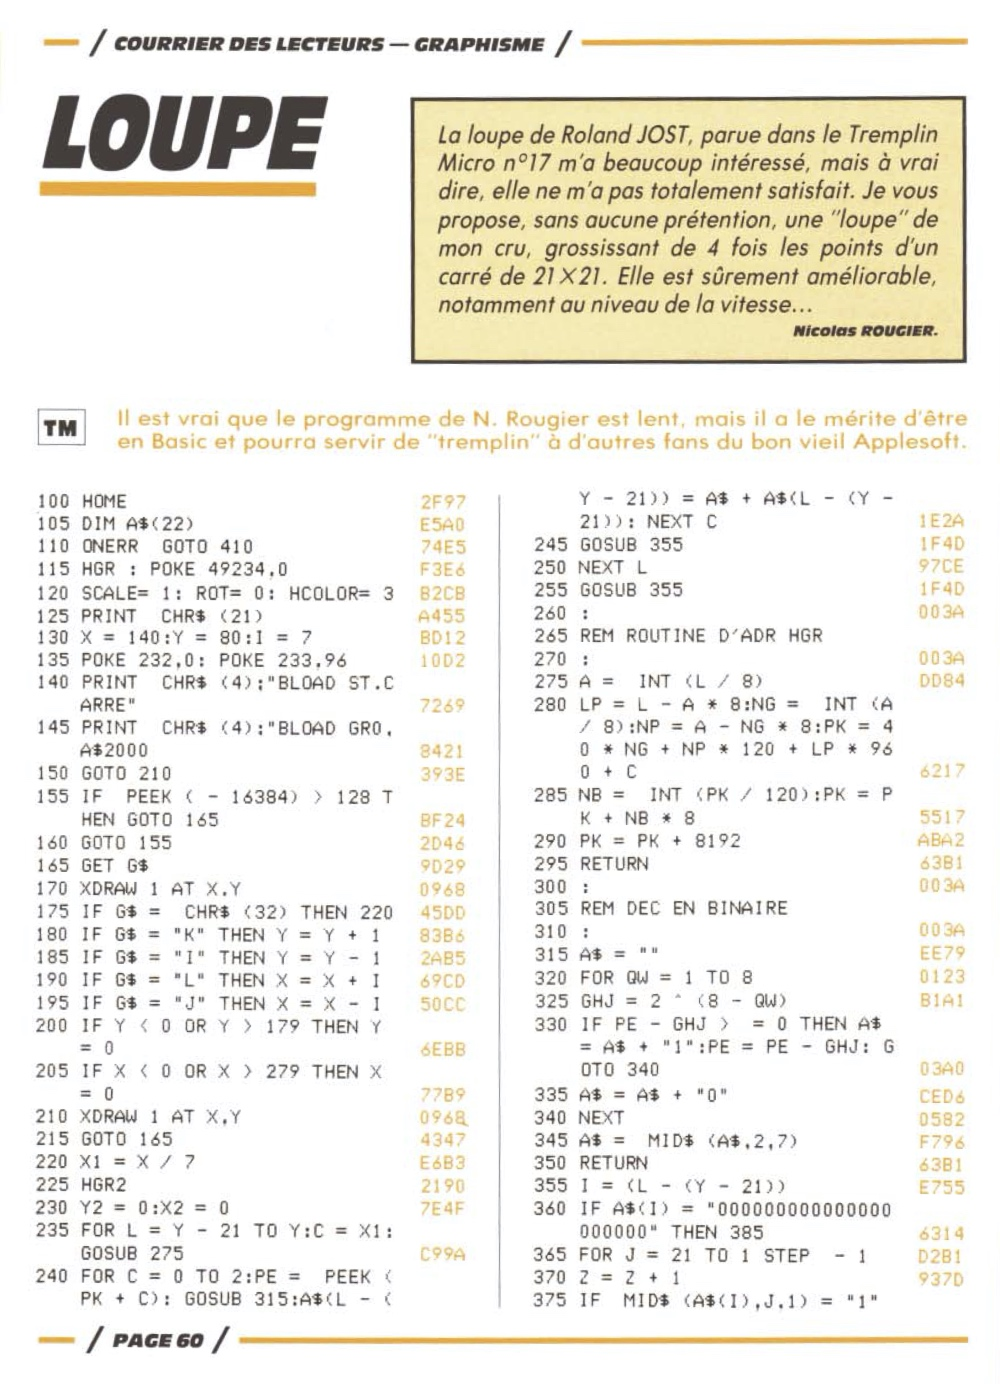
\includegraphics[width=.325\textwidth]{Tremplin-Micro-19-p60.jpg}}
\fbox{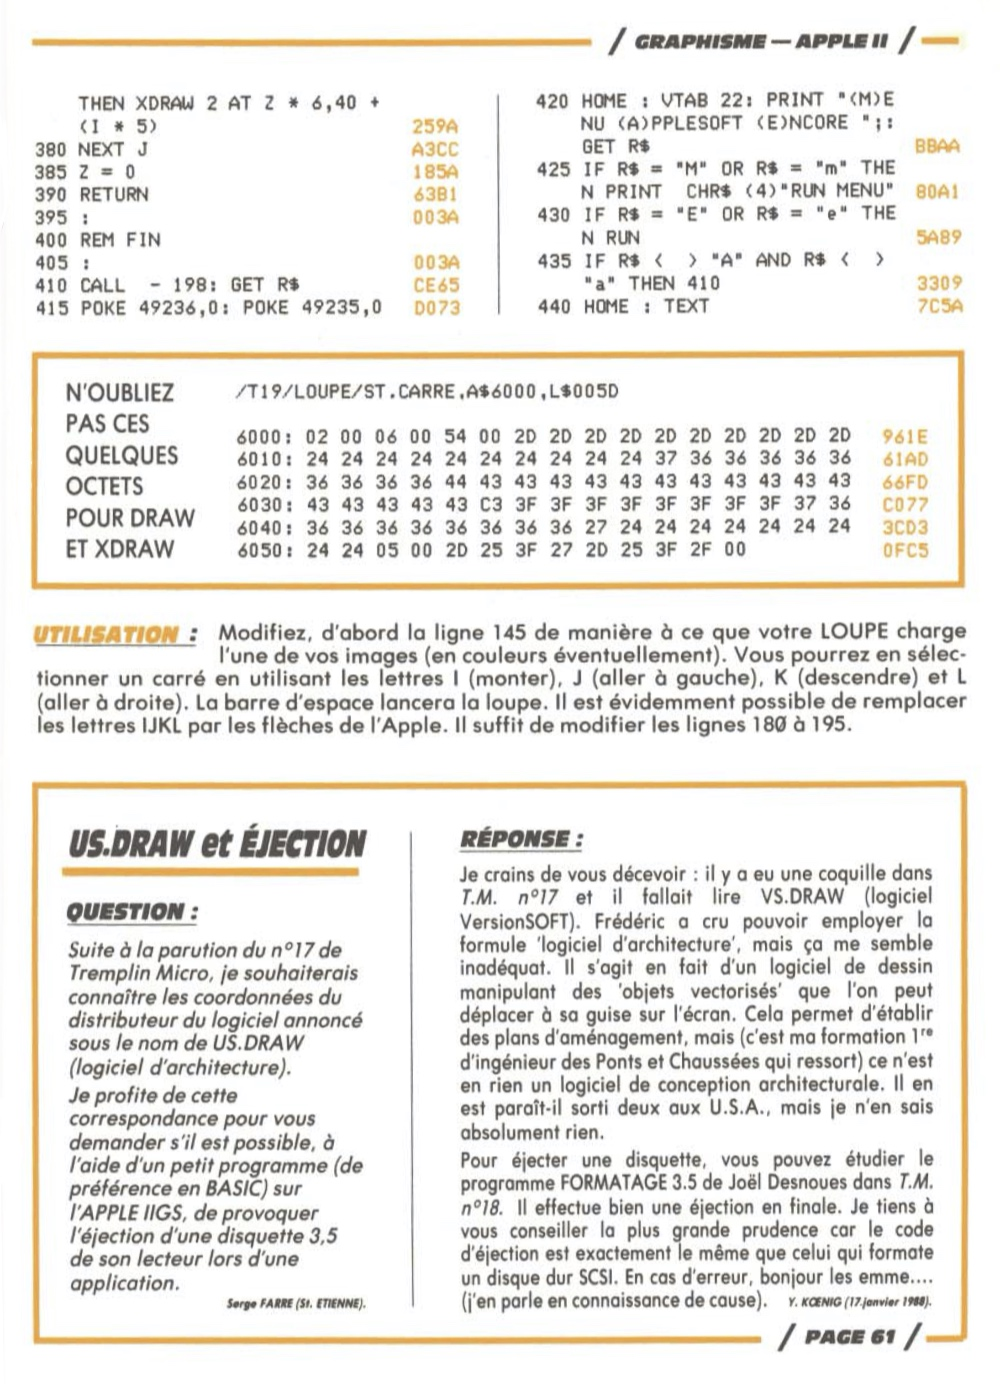
\includegraphics[width=.325\textwidth]{Tremplin-Micro-19-p61.jpg}}
}
\caption{Scans of the original magazine Tremplin Micro N$^\circ$19 (cover page,
pages 60 and 61), kindly provided by the
\href{https://archive.org/details/tremplin_micro_newsletter_issue_19}{Internet
Archive}.}
\label{fig:scans}
\end{figure}
%%
For the Ten Years Reproducibility Challenge, I thus decided to try to re-run
the original program, just for the sake of checking if I could. This includes
finding the sources (in a usable form), remembering how to load and start a
program in Applesoft, producing some original data (image) to test the program,
and of course, checking if it was running as expected.

\section*{The soft path (using an Apple~//e emulator)}

\subsection*{Looking for the sources}
I had, of course, lost track of the original sources that were saved on
5\nicefrac{\text{1}}{\text{4}} floppies and my only hope was internet. I
remembered having stumbled upon the website
\href{https://www.abandonware-magazines.org/}{Abandonware magazines}
who collect scans of French Magazine and including ``Tremplin Micro''.
(see \href{https://www.retromags.com/}{Retromags} for English magazines).
Unfortunately, the ``Tremplin Micro'' collection was not complete and I could
not find the issue where my article has been published. Fortunately, I soon
discovered other
sources\footnote{\url{http://www.apple-iigs.info/revuetremplinmicro.php}
and \url{https://archive.org/details/tremplin_micro}} and managed to find the
issue 19 (see figure~\ref{fig:scans}).

\subsection*{Transcription of the sources}
Even before asking how to run the sources, I started transcribing the scan into
a usable form (i.e. a text file) and this is the time I realized I did not know
what were the orange hexadecimal numbers for (at the right of each line). I
suspected this was some sort of checksum for controlling if what you type is
correct but I had a hard time finding the explanation on how to compute them. I
finally located the explanation on
the \href{https://archive.org/details/tremplin_micro_newsletter_issue_10/page/n3}{page
2 of issue 10}. This requires an additional program that I did not have and I
would thus not be able to control what I type.\\

The second problem was the series of hexadecimal numbers on page 61. The text
reads {\em Don't forget these few bytes for draw and xdraw}. What does that
mean? Again, I searched online for help and found that the way to use these
number is to write them directly in memory. This requires to entering the
monitor mode using the {\tt call -151} subroutine (exit with {\tt 3DOG}
or \keys{Ctrl + C} followed by \keys{\return}) and type the actual hexadecimal
numbers. For changing memory, you have to type something like:\\

\begin{tt}
] call -151\\
* 6000.6010: 02 00 06 00 54 00 2D ...\\
...\\
* 6050.605D: ...\\
* \keys{Ctrl + C} \keys{\return}\\
] BSAVE "ST.CARRE",A\$6000,L\$5D\\
\end{tt}

Since at that time I had no access to a machine, I just copied the bytes using
an hex editor and saved the result in a file named {\tt ST.CARRE}. At this
point, I had the two source files, it was time to also get some image.

\subsection*{Generating the data (image)}
For the data, I could have browsed online for some vintage Apple //e image, but
I decided instead to try to generate my own data in the native format. I
targeted
the \href{https://en.wikipedia.org/wiki/Apple_II_graphics}{High-Resolution
Graphics (HGR)} mode that has a resolution of 280$\times$192 pixels using 6
colors (with some restriction on color placement though). The corresponding
file format is really peculiar and I did not want to write my own
converter. Luckily enough, I found
the \href{http://wsxyz.net/tohgr.html}{tohgr} converter (available on mac from
the \href{https://github.com/lifepillar/homebrew-appleii}{appleii} \href{https://brew.sh/}{homebrew}
tap). This converter takes care of rescaling and dithering and also produce a
PNG image showing the result of the conversion (see
figure \ref{fig:conversion}).

\begin{figure}
{%% <-- begin a group to make \fboxsep=0pt local
\fboxsep=0pt
\fbox{
\includegraphics[width=.325\textwidth]{ReScience-original.png}}
\hfill
\fbox{
\includegraphics[width=.325\textwidth]{ReScience-screenshot-2.jpg}}
\hfill
\fbox{
\includegraphics[width=.325\textwidth]{ReScience-screenshot-1.jpg}}
}
\caption{PNG black and white image (left) converted to the HGR format
(center: monochrome, right: color) by the {\tt tohgr} program using
Floyd-Steinberg dithering.}
\label{fig:conversion}
\end{figure}


\subsection*{Running the program}

In order to run my Applesoft Basic program, I immediately thought that I would
need an emulator and this is when I discovered the huge online community that
exists around the apple //e. You have plenty of emulators available and some of
them can even be ran online through the \href{https://www.mamedev.org/}{MAME}
emulator (see for
example \href{https://archive.org/details/Karateka_1984_Broderbund}{Karateka}
by \href{https://en.wikipedia.org/wiki/Jordan_Mechner}{Jordan Mechner}
or \href{https://archive.org/details/Ultima_I_1981_California_Pacific_Computer}{Ultima
I} by \href{https://en.wikipedia.org/wiki/Richard_Garriott}{Richard
Garriott}). There even exist pure Applesoft Basic emulators\footnote{See for
example \url{https://www.calormen.com/jsbasic/}} but it is not clear how do
they interact with the machine hardware. I chose to use
the \href{http://www.virtualii.com/}{Virtual ][} by Gerard Putter who is one of
the most complete and versatile apple //e emulator. More precisely, it allows
to mount a folder as a regular disk and this offered me a way to transfer my
transcribed and generated files to the emulated machine. I then load my text
file into memory using command {\tt "LOAD LOUPE.TXT"} and it did not work, the
emulated machine choked on loading the file (I realized later that the
Applesoft Basic program were saved in a tokenized format and I should have used
the {\tt READ} command instead). I then tried to directly type the source on
the command line by copy pasting the source. To do that, I had to transform the
source such as to have every code line to fit on a single line. After doing
this, I tried to run the program using the {\tt "RUN"} command and I
immediately get my first {\tt "SYNTAX ERROR"} message (from a long suite of
future errors) accompanied by the characteristic beep signaling an error. Most
probably I did not transcribed the scan properly and I introduced some
errors.\\

\begin{figure}
{%% <-- begin a group to make \fboxsep=0pt local
\fboxsep=0pt
\fbox{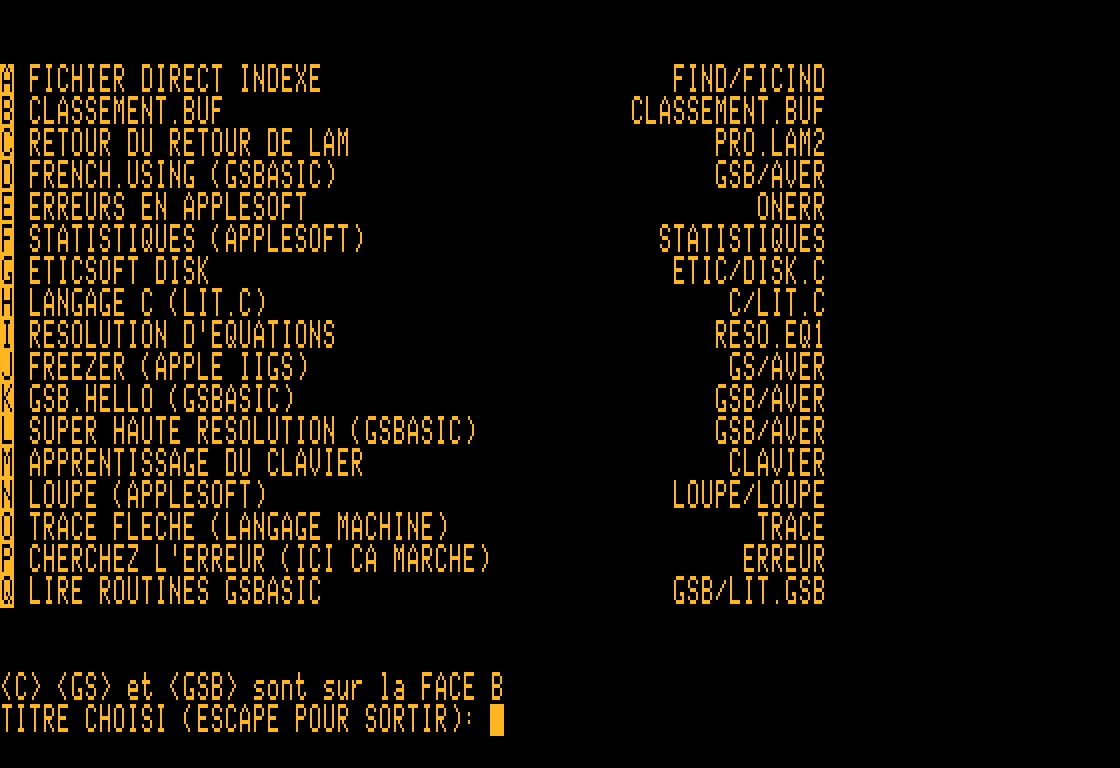
\includegraphics[width=.325\textwidth]{TM-screenshot-1.jpg}}
\hfill
\fbox{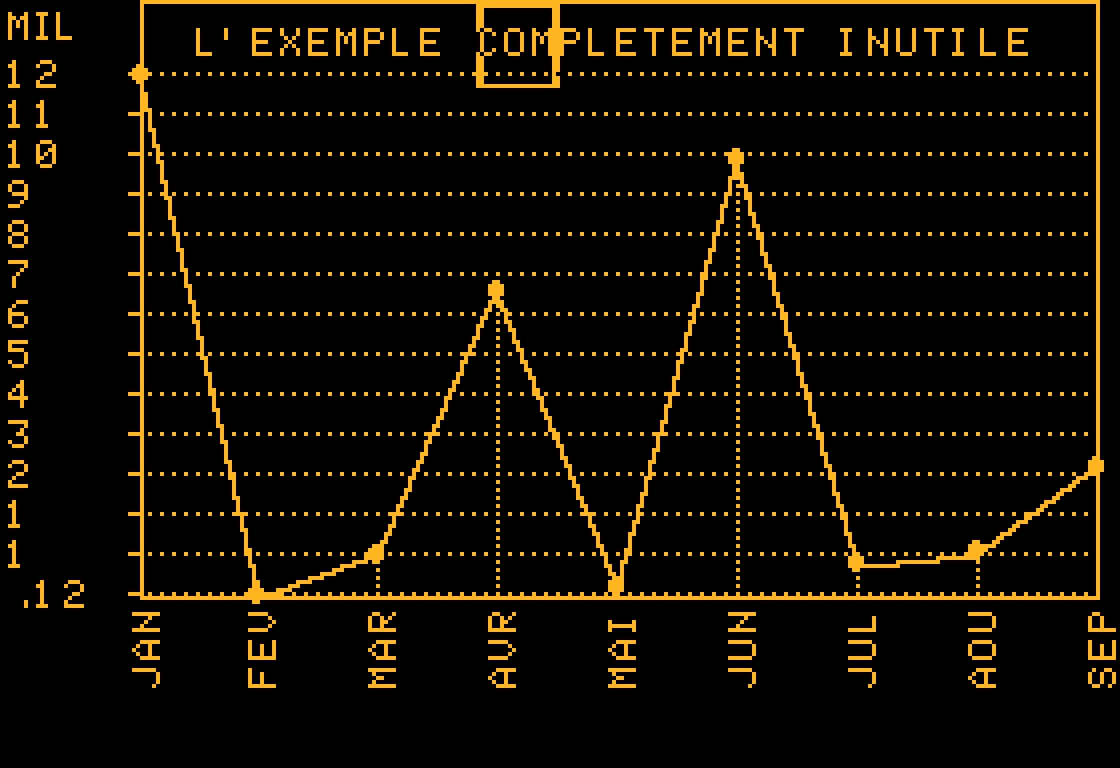
\includegraphics[width=.325\textwidth]{TM-screenshot-2.jpg}}
\hfill
\fbox{
\includegraphics[width=.325\textwidth]{TM-screenshot-3.jpg}}
}
\caption{The LOUPE program as originally distributed by the magazine on the
accompanying \href{https://mirrors.apple2.org.za/ftp.apple.asimov.net/images/non-english/french/tremplinmicro/tremplinmicro_19_disks.zip}{floppy disks}. Left: main menu (LOUPE is choice N), Center: selection of the region to zoom
(use \keys{H} \keys{I} \keys{J} \keys{K} for moving the region and \keys{<space>} for zooming out the region), Right: zoom of the selected region. }
\label{fig:original-run}
\end{figure}

Then it stroked me (rather lately) than the original magazine certainly had
accompanying floppies to save the time of typing listings for the
readers. Consequently, I searched online for the missing floppies and to my
great enjoyment, I located them in one of the biggest archive for the Apple~//e
(\href{https://mirrors.apple2.org.za}{ftp.apple.asimov.net}) that is archived at
the \href{https://archive.org/details/ftp.apple.asimov.net}{Internet Archive}
(143Go). The legal status of this archive is not clear but it seems to be
somehow tolerated and I was able to located
the \href{https://mirrors.apple2.org.za/ftp.apple.asimov.net/images/non-english/french/tremplinmicro/}{missing
floppy} saved in the common and standard {\tt dsk} format for emulators. I
then inserted the disk into the fake drive and I was able to run the program I
wrote 32 years ago (see figure \ref{fig:original-run}). Here is the full
listing (enforcing the weird and original formatting):\\

\begin{minipage}{.325\textwidth}
\begin{tiny}
\begin{framed}
\begin{verbatim}
100  HOME 
105  DIM A$(22)
110  ONERR GOTO 410
115  HGR: POKE 49234,0
120  SCALE=1: ROT=0: HCOLOR=3
125  PRINT CHR$ (21)
130  X = 140: Y = 80: I = 7
135  POKE 232,0: POKE 233,96
140  PRINT CHR$ (4);"BLOAD ST.C
     ARRE"
145  PRINT CHR$ (4);"BLOAD GR0,
     A$2000"
150  GOTO 210
155  IF PEEK ( - 16384) > 128 T
     HEN GOTO 165
160  GOTO 155
165  GET G$
170  XDRAW 1 AT X,Y
175  IF G$ = CHR$ (32) THEN 220
180  IF G$ = "K" THEN Y = Y + 1
185  IF G$ = "I" THEN Y = Y - 1
190  IF G$ = "L" THEN X = X + I
195  IF G$ = "J" THEN X = X - I
200  IF Y < 0 OR Y > 179 THEN Y
     = 0
205  IF X < 0 OR X > 279 THEN X
     = 0
210  XDRAW 1 AT X,Y
215  GOTO 165
220  X1 = X / 7
225  HGR2
\end{verbatim}
\vspace{-2\baselineskip}
\end{framed}
\end{tiny}
\end{minipage}
%
\hfill
%
\begin{minipage}{.325\textwidth}
\begin{tiny}
\begin{framed}
\begin{verbatim}
230  Y2 = 0:X2 = 0
235  FOR L = Y - 21 TO Y:C = X1:
     GOSUB 275
240  FOR C = 0 TO 2:PE =  PEEK (
       PK + C): GOSUB 315:A$(L-(
       Y - 21)) = A$ + A$(L -(Y-
       21)):NEXT C
245  GOSUB 355
250  NEXT L
255  GOSUB 355
260  :
265  REM  ROUTINE D'ADR HGR
270  :
275  A  = INT (L / 8)
280  LP = L - A * 8: NG = INT (A
     / 8):NP = A - NG * 8:PK = 4
     0 * NG + NP * 120 + LP * 96
     0 + C
285  NB =  INT (PK / 120):PK = P
     K + NB * 8
290  PK = PK + 8192
295  RETURN 
300  :
305  REM  DEC EN BINAIRE
310  :
315  A$ = ""
320  FOR QW = 1 TO 8
325  GHJ = 2 ^ (8 - QW)
330  IF PE - GHJ > = 0 THEN A$
     = A$ + "1":PE = PE - GHJ: G
     OTO 340
\end{verbatim}
\vspace{-2\baselineskip}
\end{framed}
\end{tiny}
\end{minipage}
%
\hfill
%
\begin{minipage}{.325\textwidth}
\begin{tiny}
\begin{framed}
\begin{verbatim}
335  A$ = A$ + "0"
340  NEXT 
345  A$ = MID$ (A$,2,7)
350  RETURN 
355  I = (L - (Y - 21))
360  IF A$(I) = "00000000000000
     0000000" THEN 385
365  FOR J = 21 TO 1 STEP - 1
370  Z = Z + 1
375  IF MID$ (A$(I),J,1) = "1"
     THEN XDRAW 2 AT Z * 6,40 +
     (I * 5)
380  NEXT J
385  Z = 0
390  RETURN 
395  :
400  REM   FIN
405  :
410  CALL - 198: GET R$
415  POKE 49236,0: POKE 49235,0
420  HOME : VTAB 22: PRINT "(M)E
     NU (A)PPLESOFT (E)NCORE ";:
     GET R$:
425  IF R$ = "M" OR R$ = "m" THE
     N PRINT CHR$(4) "RUN MENU"
430  IF R$ = "E" OR R$ = "e" THE
     N RUN 
435  IF R$ < > "A" AND R$ < > 
     "a" THEN 410
440  HOME: TEXT

\end{verbatim}
\vspace{-2\baselineskip}
\end{framed}
\end{tiny}
\end{minipage}

\subsection*{Making a floppy image}

The last step in my journey was to make a bootable floppy image that could be
used by a neophyte user. This took me some time to find the relevant command
({\tt INIT HELLO}) for making a bootable disk (that executes the {\tt HELLO}
program when booted). With the help of the Virtual ][ emulator, it was then easy
to convert the mounted folder into
a \href{http://fileformats.archiveteam.org/wiki/DSK_(Apple_II)}{dsk} image
which is one the standard disk format for the Apple~//e. The image is provided
in the GitHub repository and can be ran with the excellent \href{https://www.scullinsteel.com/apple/e}{Apple//jse emulator} by Will Scullin. You should obtain the results shown on figure \ref{fig:disk-screenshots}.

\begin{figure}
{%% <-- begin a group to make \fboxsep=0pt local
\fboxsep=0pt
\fbox{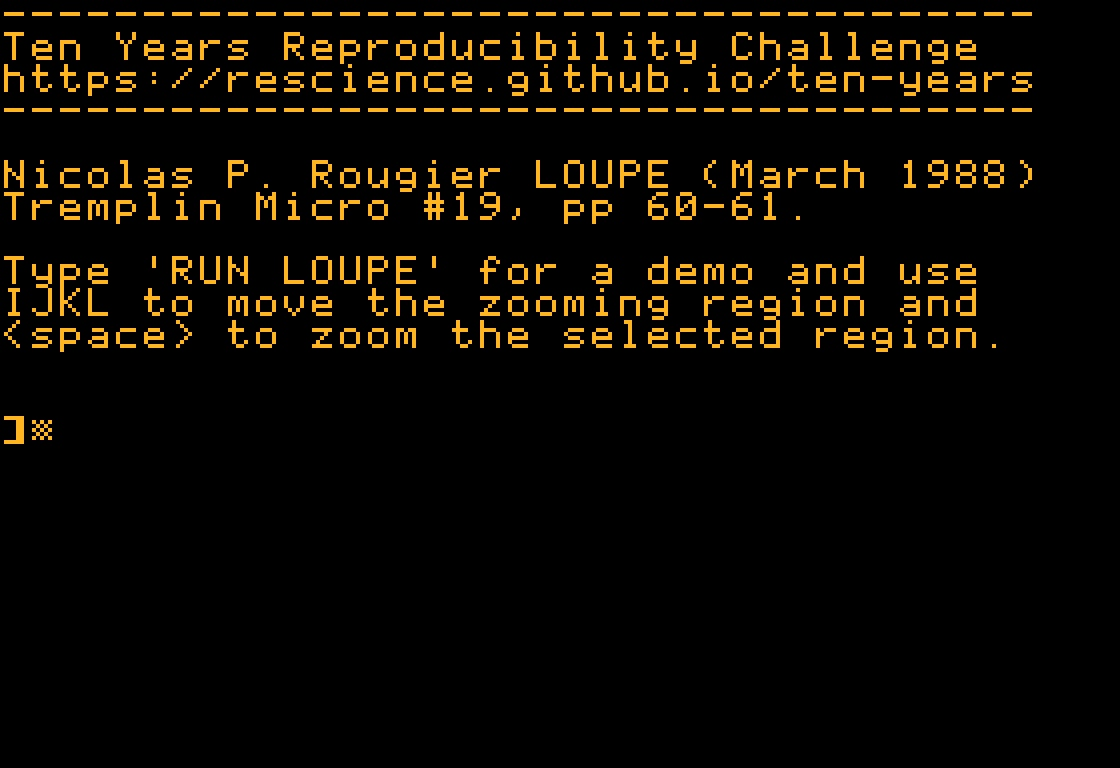
\includegraphics[width=.325\textwidth]{disk-screenshot-1.jpg}}
\hfill
\fbox{
\includegraphics[width=.325\textwidth]{disk-screenshot-2.jpg}}
\hfill
\fbox{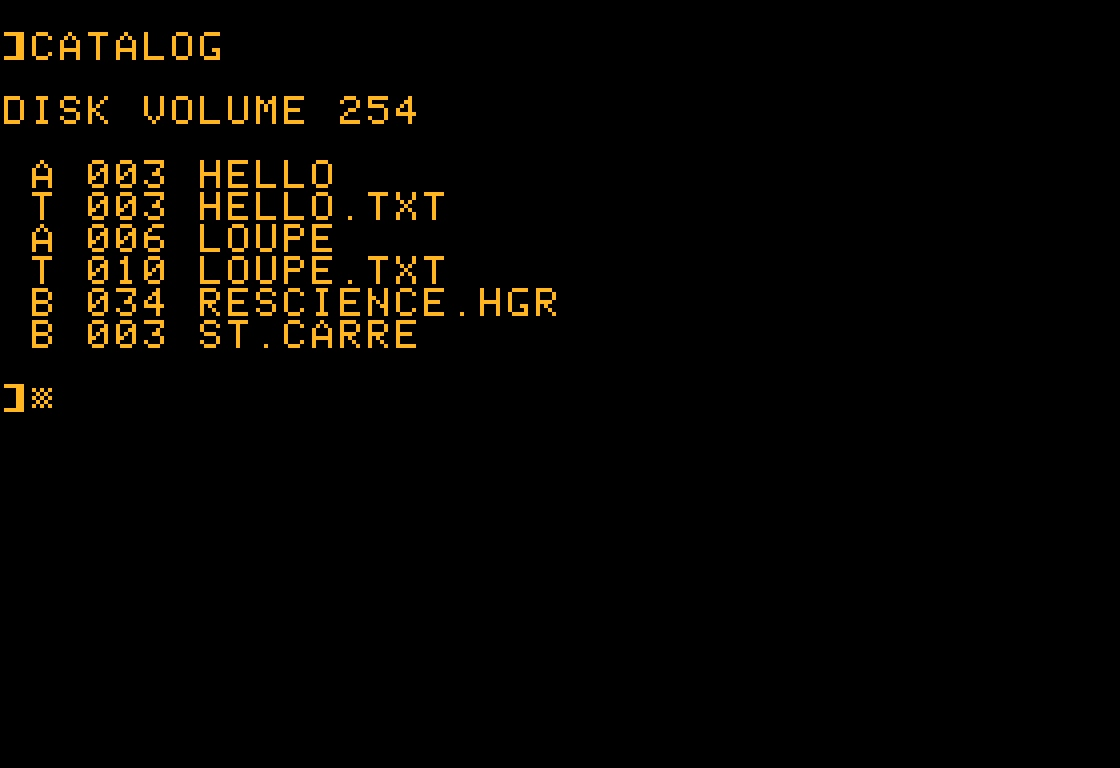
\includegraphics[width=.325\textwidth]{disk-screenshot-3.jpg}}
}
\caption{Screenshots of the final floppy image with the LOUPE program. The image can be used with most Apple //e emulators.}
\label{fig:disk-screenshots}
\end{figure}


\section*{The hard path (using a vintage apple //e machine)}

Once I've produced the disk image, I decided I could try to write it onto a
real \href{https://en.wikipedia.org/wiki/History_of_the_floppy_disk}{floppy}
since it happens that I've a vintage Apple~//e machine in my office. First
thing to do was to find a 5\nicefrac{\text{1}}{\text{4}} floppy drive that can
be connected through a modern interface such as USB. Surprisingly enough, there
are none, or at least, I did not find them. The solution was then to connect
one of the external drive of the Apple~//e to the USB port using an external
controller. I found the
\href{https://applesaucefdc.com/}{Applesauce floppy drive controller} with
the associated software to be among the best (and probably one of the most
expensive) solution. Second step was to acquire ``brand new'' floppy disks and
again, I was surprised, but this time, by the plethora of vintage floppies you
can buy online. I bought a box of 10 floppies dated back to 1992. I then wrote
the image to one floppy (three times in a row because the floppy were quite
old) and I booted the machine with the floppy. The final result is shown on figure \ref{fig:final}.
%
\begin{figure}
{%% <-- begin a group to make \fboxsep=0pt local
\fboxsep=0pt
\fbox{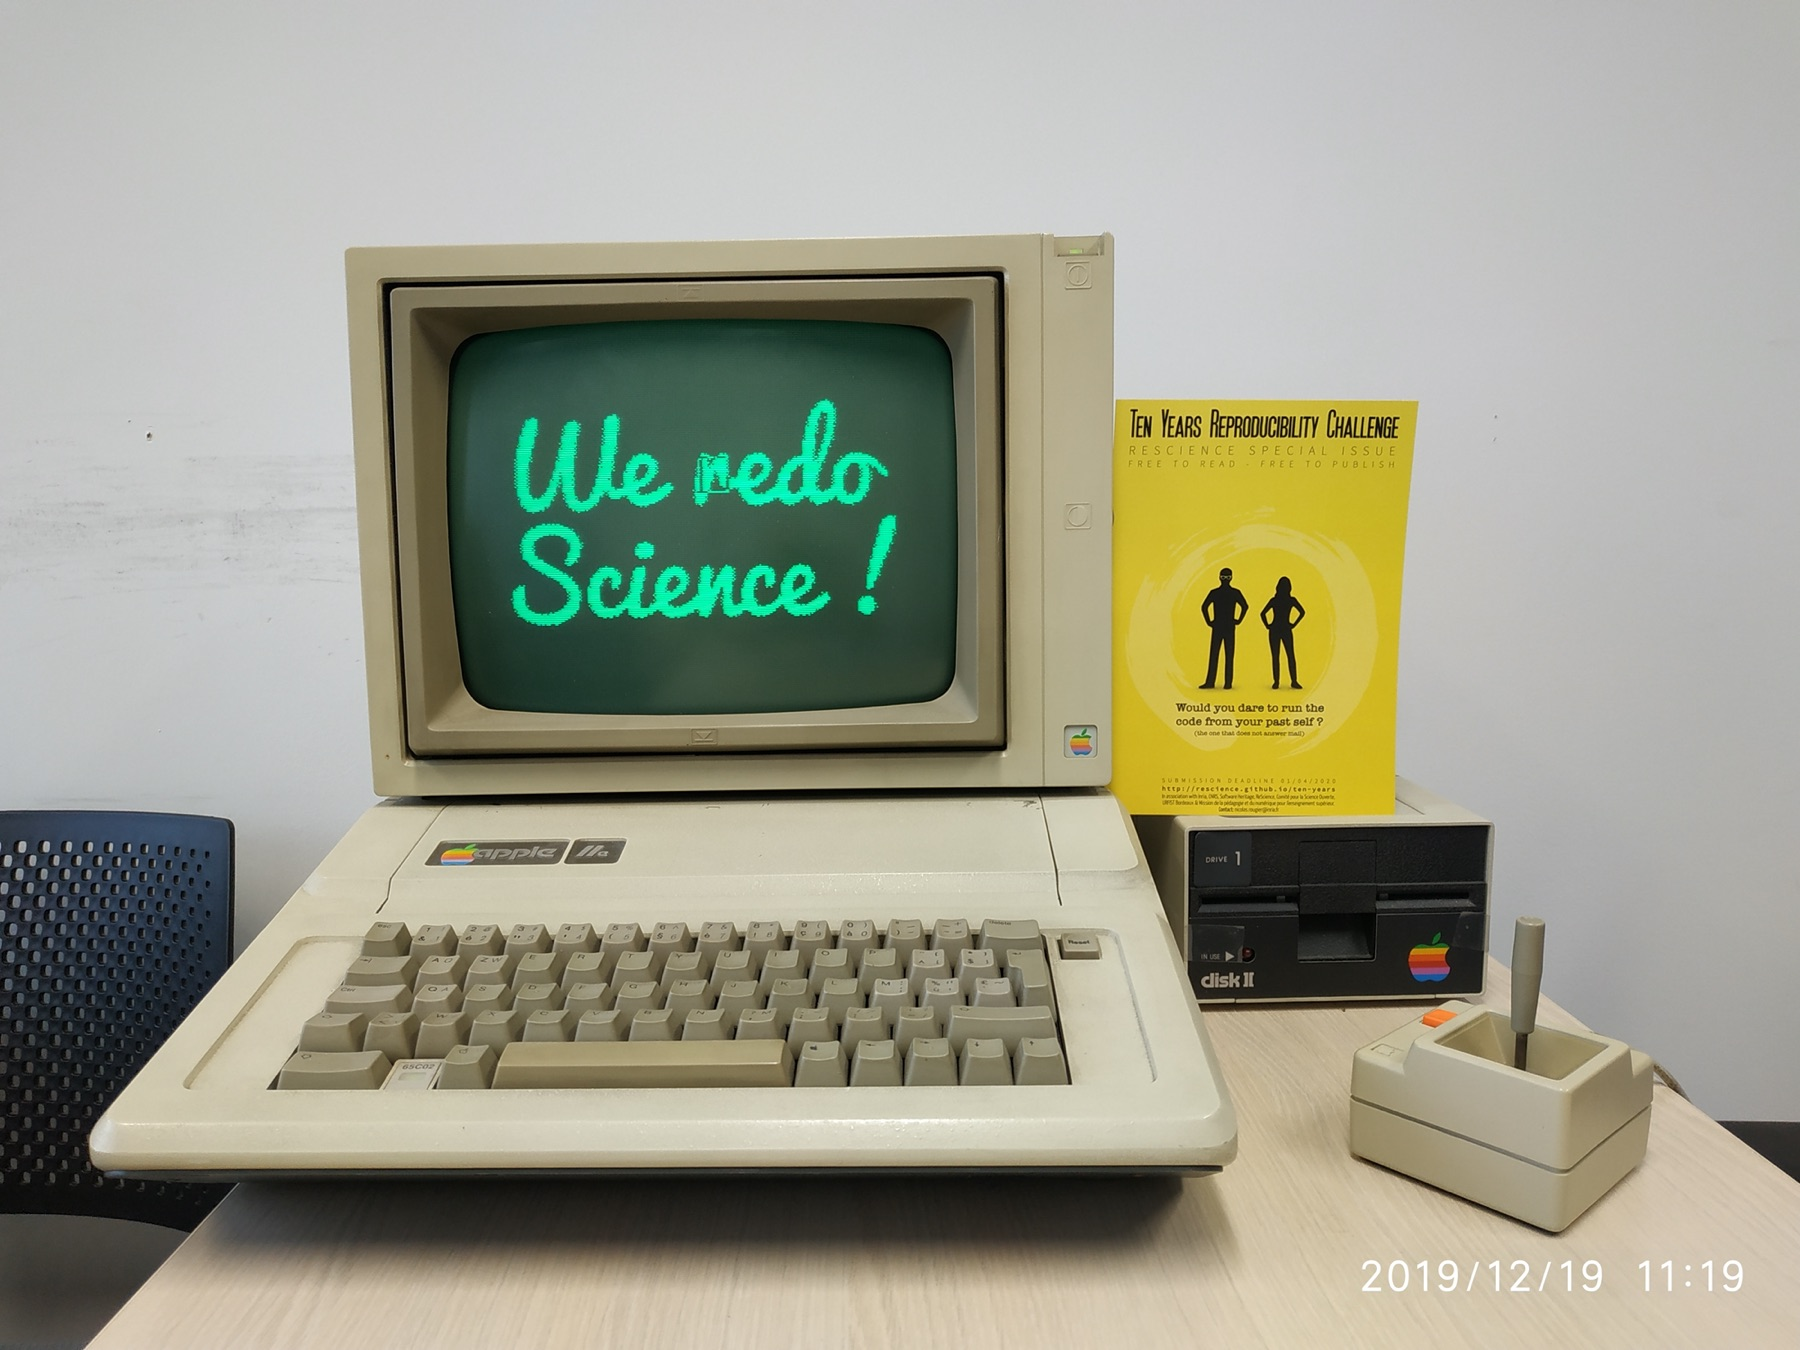
\includegraphics[height=6.35cm]{NPRougier_2019-Dec-19-1.jpg}}
\hfill
\fbox{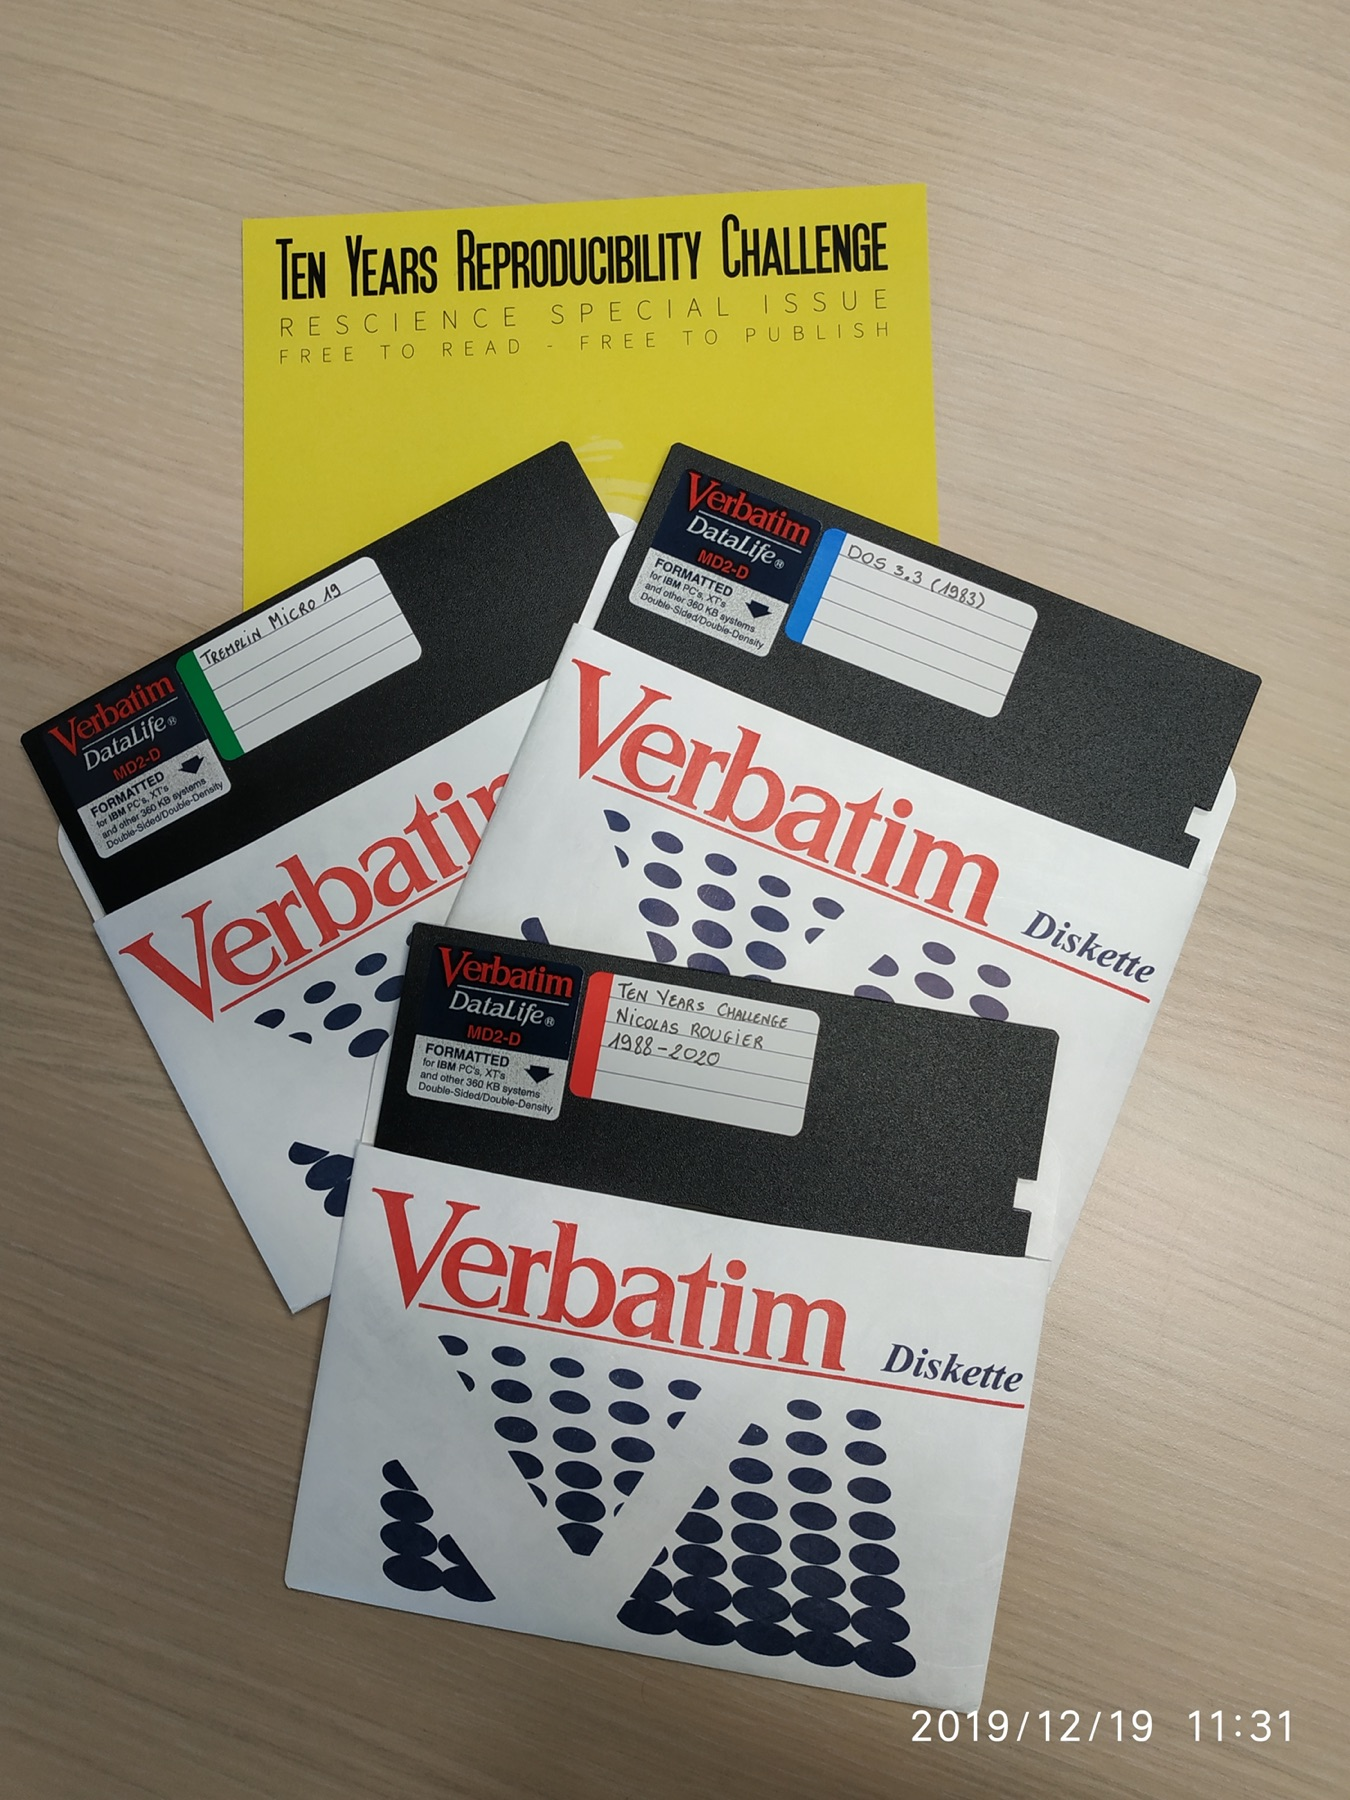
\includegraphics[height=6.35cm]{NPRougier_2019-Dec-19-2.jpg}}
}\\
\caption{The original LOUPE program running on a vintage Apple //e with brand new data}
\label{fig:final}
\end{figure}

Of course, and because I now had a usable drive, I search thoroughly for my
original floppies and eventually found them. Even after having spent 30 years
in a non-heated attic while being loosely protected, most of them were still
readable. I found the original sources of the LOUPE program as well as earlier
versions using a primitive versioning system ({\tt LOUPE1.BAS and LOUPE2.BAS,
etc}).\\

I can now declare my challenge completed and successful!

\subsection*{Usage}

If you want to quickly test the program, go to
the \href{https://www.scullinsteel.com/apple2/}{Apple2JS emulator} website and
load the disk image available from \url{https://github.com/rougier/TYRC-apple}
and follows on-screen instructions.

\section*{Discussion}

Even though the original article was not scientific, the experience was
nonetheless challenging, interesting and instructive. Challenging because I
barely remembered most of the commands I used to type all night long 32 years
ago but, as soon as I started to play again with the emulator, I rapidly
recover most of my old habits. For the rest, there are the various pieces of
documentation you can easily find online, from the scan of the original
documentations accompanying the Apple //e, the various books that have been
written on the matter, the various Wikipedia dedicated pages and the incredibly
large number of resources that have been written by Apple enthusiasts. Taken
together, this represents a precious knowledge for the future.\\

It was also quite interesting, as well as really surprising, to discover that
hardware is still being developed for this 40 years old (but quite) robust
machine. For example, the floppy drive controller I've acquired has been
released in 2018 and website such
as \href{https://www.a2heaven.com}{a2heaven.com} are still developing news
cards for the hobbyists. Furthermore, the machine in my office is working like a
charm and most of the floppies I tried to run have been working without a
glitch. It seems that floppy disks area actually quite a reliable storage
medium. According to the \href{http://www.softpres.org/}{Software Preservation
Society}, their lifespan ranges from 10 to 30 years depending on storage
condition\supercite{lowood:2009}. From my own experience, I can only confirm
these numbers.\\

The whole experience has been also quite instructive when compared to modern
research practices. Despite minor problems, my experience has been rather
smooth (and fun) and I think the main reason for such smoothness lies in the
closed and frozen nature of the target. Applesoft Basic was proprietary and
there have been only two versions, the first one was on tape and available with
the original Apple II while the second and more widespread version was either
built into the ROM of (since the ][+) or available with DOS 3.3 and ProDOS's
BASIC.SYSTEM. This means the syntax of the Applesoft Basic never really changed
over (almost) 15 years, from 1979 to 1993 when Apple stopped shipping the
Apple~II. Same is true for the 6502 microprocessor that only evolved to the
65C02 with the Apple IIc but remains largely compatible with the 6502. Such
stability undoubtedly gave time to developpers to really exploit the machine
and pushed it to its limits. See for example
the \href{https://retroconnector.com/mining-bitcoin-on-an-apple-ii-a-highly-impractical-guide/}{
Mining Bitcoin on an Apple II, a highly impractical guide}. If you compare this
non-evolutive platform to the current situation of programming languages (where
it is not rare to have several minor releases in a year with potential
deprecations), you cannot help to think that doing the same challenge ten years
from now will be much more difficult.\\

Finally, I cannot help to compare Applesoft Basic with the Python language
whose version 2 will hit end of life on January 1, 2020. Of course, we've been
warned a long time ago and we had plenty of time to prepare for the change. But
still, it will undoubtedly break things in the short term and probably even more
things in the long term. And yet, this end of life might be a good thing for
Science because we now have at our disposal an \textbf{advanced programming
language that is guaranteed not to evolve anymore} (i.e. Python 2.7). We may
very well have a modern equivalent of the late Applesoft Basic that proved
itself to be a highly fertile ground for development. Of course, we won't
benefit from the latest and most advanced features of Python 3, but do we
really need them?  Considering myself as a Scientific Python expert, I know
that I'm not using 90\% of the Python 3 new features and I suspect I'm not the
only one. Overall, a {\em dead language} such a Python 2 might represent a real
opportunity for Science. Who knows?


\section*{Resources}

Here is a partial list of resources I've used during the Challlenge:
\begin{itemize}
\item \href{http://www.virtualii.com/}{Virtual ][}: application that emulates the vintage Apple II computer (Mac).
\item \href{https://applesaucefdc.com/}{Applesauce}: floppy drive controller
for Apple ][ 5.25″ drive (Mac).
\item \href{https://github.com/dmolony/DiskBrowser}{Apple II disk browser}: browser content of disk images.
\item \href{https://mirrors.apple2.org.za/ftp.apple.asimov.net/}{ftp.apple.asimov.net}: main repository of disk images for the Apple 2.
\item \href{http://wsxyz.net/tohgr.html}{tohgr}: convert images in PNG/JPG format to Apple II images. 
\end{itemize}

